%-----------------------------------------------------------------------------
%
%               Template for sigplanconf LaTeX Class
%
% Name:         sigplanconf-template.tex
%
% Purpose:      A template for sigplanconf.cls, which is a LaTeX 2e class
%               file for SIGPLAN conference proceedings.
%
% Guide:        Refer to "Author's Guide to the ACM SIGPLAN Class,"
%               sigplanconf-guide.pdf
%
% Author:       Paul C. Anagnostopoulos
%               Windfall Software
%               978 371-2316
%               paul@windfall.com
%
% Created:      15 February 2005
%
%-----------------------------------------------------------------------------


\documentclass[preprint]{sigplanconf}

% The following \documentclass options may be useful:

% preprint      Remove this option only once the paper is in final form.
% 10pt          To set in 10-point type instead of 9-point.
% 11pt          To set in 11-point type instead of 9-point.
% authoryear    To obtain author/year citation style instead of numeric.

\usepackage{amsmath,amssymb}
\usepackage[T1]{fontenc}
\usepackage{filecontents}
\usepackage{hyperref}
\usepackage{graphicx}
\usepackage{float}
\usepackage[note]{marginote} % remove before sending.

\begin{filecontents}{workshop.bib}
@Manual{Coq,
  title =        {The {Coq} Proof Assistant Reference Manual},
  author =       {{The Coq Development Team}},
  organization = {{LogiCal} Project},
  note =         {Version 8.0},
  year =         {2004},
  url =          "http://coq.inria.fr"
}

@InCollection{ProofGeneral,
  Title                    = {Proof General: A Generic Tool for Proof Development},
  Author                   = {Aspinall, David},
  Booktitle                = {Tools and Algorithms for the Construction and Analysis of Systems, {TACAS} 2000},
  Publisher                = {Springer Berlin Heidelberg},
  Year                     = {2000},
  Editor                   = {Graf, Susanne and Schwartzbach, Michael},
  Pages                    = {38--43},
  Series                   = {Lecture Notes in Computer Science},
  Volume                   = {1785},
  Doi                      = {10.1007/3-540-46419-0_3},
  ISBN                     = {978-3-540-67282-1},
  Language                 = {English},
  Url                      = {http://dx.doi.org/10.1007/3-540-46419-0_3}
}

@Electronic{SMIE,
  Title                    = {{SMIE: Simple Minded Indentation Engine}},
  Author                   = {Stefan Monnier},
  Url                      = {https://www.gnu.org/software/emacs/manual/html_node/elisp/SMIE.html},
  Year                     = {2010}
}
\end{filecontents}

\usepackage{xspace}
% To have the same capitalization everywhere
\newcommand{\proofg}{\emph{Proof General}\xspace}
\begin{document}

\special{papersize=8.5in,11in}
\setlength{\pdfpageheight}{\paperheight}
\setlength{\pdfpagewidth}{\paperwidth}

\conferenceinfo{CoqPL 2016}{January 23, 2016, St. Petersburg, Florida, United States}
\copyrightyear{2016}
% \copyrightdata{978-1-nnnn-nnnn-n/yy/mm}
% \doi{nnnnnnn.nnnnnnn}

% Uncomment one of the following two, if you are not going for the 
% traditional copyright transfer agreement.

%\exclusivelicense                % ACM gets exclusive license to publish, 
                                  % you retain copyright

%\permissiontopublish             % ACM gets nonexclusive license to publish
                                  % (paid open-access papers, 
                                  % short abstracts)

\titlebanner{}        % These are ignored unless
\preprintfooter{Company-Coq: Taking Proof General one step closer to a real IDE}   % 'preprint' option specified.

\title{Company-Coq: Taking Proof General one step closer to a real IDE}
\subtitle{A tutorial on using Proof General and its new extension to write proofs more efficiently}

\authorinfo{Cl�ment Pit-Claudel}
           {MIT CSAIL}
           {cpitcla@mit.edu}
\authorinfo{Pierre Courtieu}
           {CNAM, Lab. C�dric}
           {pierre.courtieu@cnam.fr}

\maketitle

\begin{abstract}
\texttt{Company-Coq} is a new Emacs package that extends \proofg with a contextual auto-completion engine for Coq proofs and a many additional facilities to make writing proofs easier and more efficient. Beyond fuzzy auto-completion of tactics, options, module names, and local definitions, \texttt{company-coq} offers offline in-editor documentation, convenient snippets, and many other Coq-specific IDE features. The presentation will focus on a live demo of the system with an emphasis on writing proofs in Emacs more efficiently, and a discussion of desirable features of proof-oriented development environments.
\end{abstract}

\category{D.2.6}{Software Engineering}{Programming Environments---Integrated environments}

\terms Verification

\keywords IDE, documentation, proof engineering, user experience

\section*{Introduction}

Users of the Coq Proof Assistant \cite{Coq} are roughly divided between two interactive development environments\footnote{There also exists Coq interfaces for vim and Eclipse, though their use does not seem very widespread}: \proofg, an extension of of Emacs written by David Aspinall et al. \cite{ProofGeneral}, and \emph{CoqIDE}, a Coq-specific development environment written from scratch by members of the Coq team and generally touted as more beginner-friendly (mostly due \proofg's dependence on Emacs). Both are powerful tools for writing proofs, and significantly improve the experience of proof authors when compared to Coq's simple read-eval-print loop. Yet these tools do not offer advanced features typically found in IDEs like Eclipse or Visual Studio, such as in-editor documentation or context-sensitive completion. In addition, when advanced features are in fact available (Proof General, for example, does supports snippets and improved display of mathematics), they tend to lack discoverability: users do not explore the menus and miss convenient features that would make them more efficient.

\section*{Workshop description}

The workshop will consist in a quick run through \texttt{company-coq} features, and a tutorial on using these and other Proof General features to write proofs more efficiently. We will put emphasis on the lemma extraction feature in particular, showing how it can be used to structure proof developments more clearly. More generally, the workshop will also be a good occasion to showcase some features that \emph{Proof General} inherits from Emacs, and discuss how much of this work could be used to enhance other Coq interfaces. In particular, the development of \texttt{company-coq} has resulted in the manual annotation of the user manual to extract tactic templates and the associated documentation; the resulting list of tactics could be useful to other editors.

\section*{Overview of some features of \texttt{company-coq}}

\texttt{Company-Coq} is a new Emacs package that attempts to fix some of these limitations: it extends \proofg with many advanced IDE features (such as fuzzy completion, various Coq-specific snippets, and in-editor documentation for most of Coq's 2000-odd tactics, options, and errors), and it solves the discoverability issue by taking an ``all-on'' approach where the default distribution has most features automatically enabled. In addition, \texttt{company-coq} comes with a comprehensive tutorial that showcases most of its features. Some examples include:

\paragraph{Context-sensitive autocompletion with holes} \texttt{Company-Coq} implements a number of backends for the \emph{CompleteAnything} Emacs package (\texttt{company}). Typing \texttt{appl{\kern0.1pt}in} therefore suggests variants of the apply tactic:

\begin{figure}[H]
  \centering
  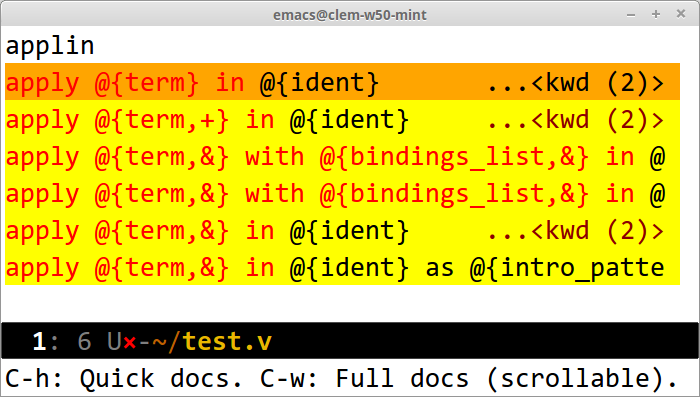
\includegraphics[width=\linewidth]{apply-in-xxl.png}
\end{figure}

\paragraph{Offline documentation lookups} Part of the development of \texttt{company-coq} involved cross-referencing all tactics from the user manual; this, in turns, allows \texttt{company-coq} to display documentation for most completion entries:

\begin{figure}[H]
  \centering
  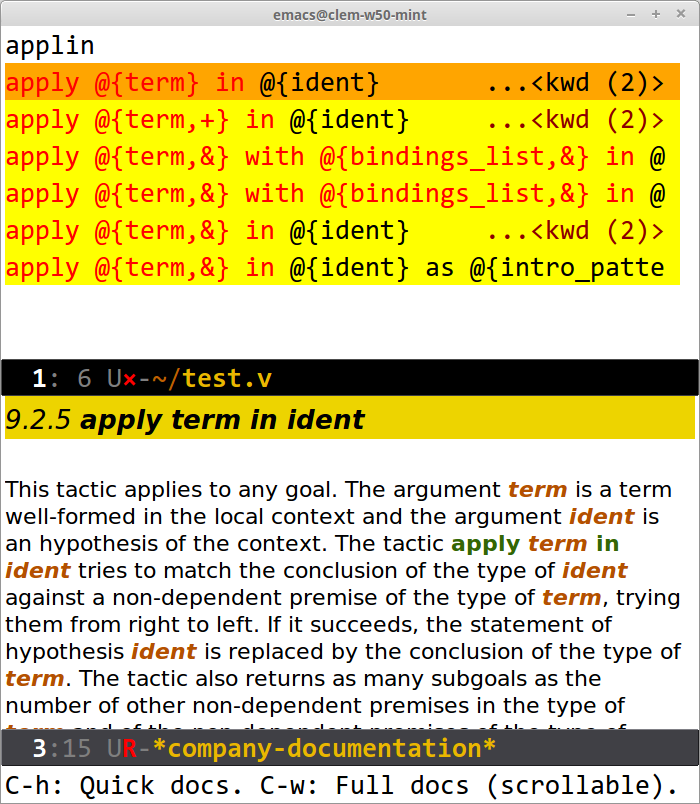
\includegraphics[width=\linewidth]{docs-xxl.png}
\end{figure}

\paragraph{Lemma extraction} At any point in a proof, users may choose to extract the current goal, including relevant hypotheses, to a separate lemma. Instead of painstakingly copy-pasting the relevant hypotheses, \texttt{company-coq} offers a convenient interface to pick relevant hypotheses and generate the statement of the new lemma.

\paragraph{Point and click documentation} Clicking on an identifier while pressing the control key opens an inline documentation window:

\begin{figure}[H]
  \centering
  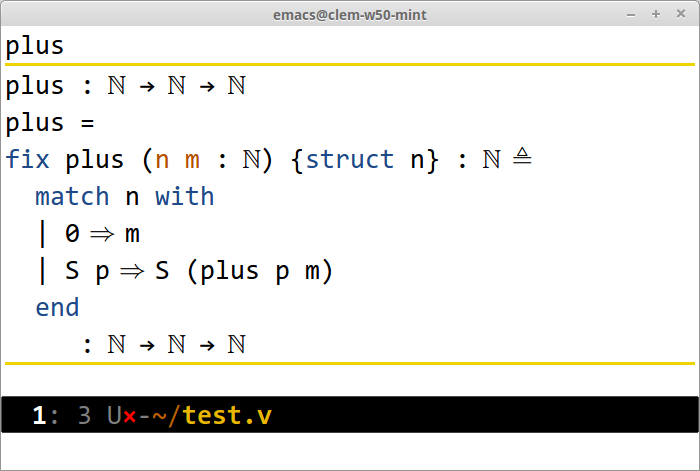
\includegraphics[width=\linewidth]{inline-docs-xxl.png}
\end{figure}

\paragraph{Snippets} \texttt{Company-Coq} connects with \texttt{YASnippet} to make certain common Coq patterns quicker to write. For example, to write
\begin{verbatim}
match goal with
| [ H: ?a /\ ?b |- ?a ] => destruct H; assumption
end
\end{verbatim}
the user need only type
\begin{verbatim}
mgw RET
M-S-RET TAB ?a /\ ?b TAB ?a TAB
destr RET H; ass RET
\end{verbatim}
the key here is the \texttt{M-S-RET} shortcut, which introduces the
\begin{verbatim}
| [ H: _ |- _ ] => _
\end{verbatim}
pattern, leaving holes that the user can navigate between with \texttt{TAB} in place of each \texttt{\_}.

\paragraph{Automatic named introduction} Scripts that depend on the name of hypotheses can often be made more robust by choosing names explicitly: \texttt{company-coq} leverages an existing feature of \proofg to let the user type
\begin{verbatim}
intros! RET
\end{verbatim}
to create an invocation of the \texttt{intros} tactic that explicitly mentions all introduced variables, using Coq's \emph{Smart intros} feature.

\section*{New features of \proofg}

A number of new Proof General features are also useful for proof development:

\paragraph{Automatic indentation of bulleted proofs} Coq proofs can be structured with \emph{bullets} and curly brackets, making proof structure more readily apparent, and helping with maintenance. Thanks to \texttt{SMIE} \cite{SMIE}, an Emacs indentation package, \proofg implements an indentation routine based on structuring commands which makes proofs easier to format.

\paragraph{Automatic recompilation at \texttt{Require}} When developing a proof, one has to deal with several inter-dependent files. \proofg, thanks to a contribution of Hendrik Tews, can transparently and recursively recompile dependencies as it reaches \texttt{Require} commands, launching the required compilation jobs in the background.

% Je laisse �a de c�t� vu aue ce n'est pas encore impl�ment� dans Company-Coq :)
% In the same spirit some tactics come with the ability to name the created hypothesis (\texttt{induction ... as ..., inversion ... as ..., \ldots}) \proofg comes with a facility to automatically generate the \texttt{as} closes and \texttt{Company-Coq}\marginote{\`a implanter/changer} bring this feature to the user as an auto-completion of the keyword \texttt{as!}.

\section*{Conclusion}
Since it is not part of the core \emph{Proof General}, \texttt{company-coq} can be used as a convenient area to test new IDE features before they are merged into Proof General or CoqIDE, and discuss new development directions: for example, although \emph{Proof General} does support enhanced displaying of mathematics (non-destructively showing \texttt{fun (n m: nat) => forall p, p <> n -> p >= m} as \texttt{$\lambda$ (n m: $\mathbb N$) $\Rightarrow$ $\forall$ p, p $\neq$ n $\rightarrow$ p $\geq$ m}), few users seem to know about that feature. \texttt{Company-Coq}, on the other hand, enables a similar feature by default, and most users seem pleased with it. We hope that the CoqPL workshop will be a good venue to discuss the development of new editor features to support the accelerated development of Coq programs and proofs.

\bibliographystyle{abbrvnat}
\bibliography{workshop}

\end{document}
